\newpage
\section{RESULT}
\subsection{Big Five Personality Frequency Distribution}
myPersonality dataset contains status updates of 223 users. These users come under Big Five Personality traits. We analyzed this data to see how users are distributed under different personality traits. The frequency distribution of each class of personality traits is given below:
\begin{figure}[!ht]
\centering
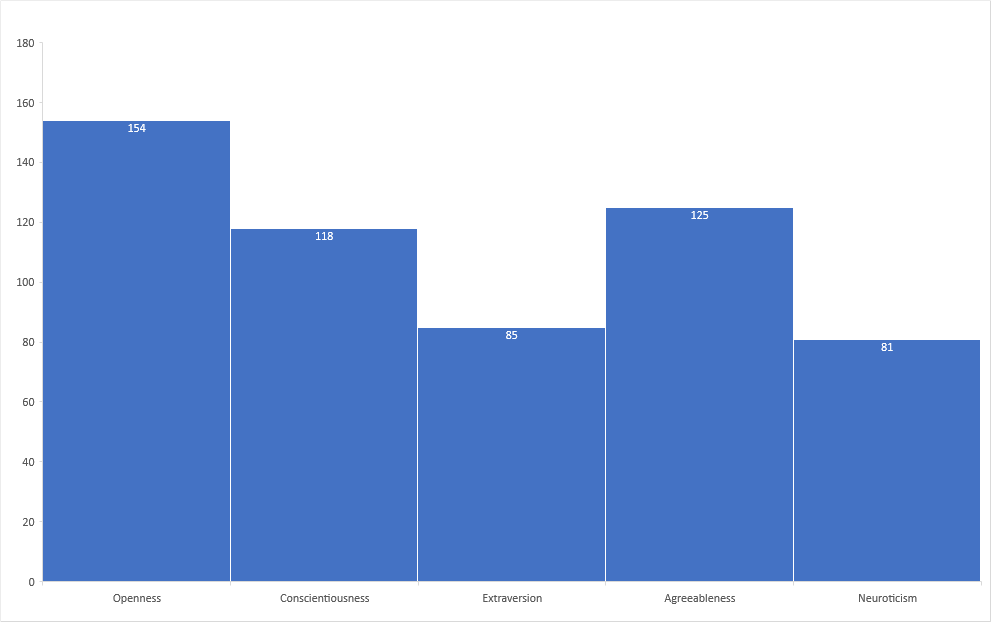
\includegraphics[width = \textwidth ]{fig/class_frequency.png}
\caption{Class Frequency Distribution of Users}
\label{fig:class_frequency}
\end{figure}

\subsection{Logistic Regression Model}
We analyzed the effect of number of iterations on the f-measure of the logistic regression model which is given below:
\begin{figure}[!ht]
\centering
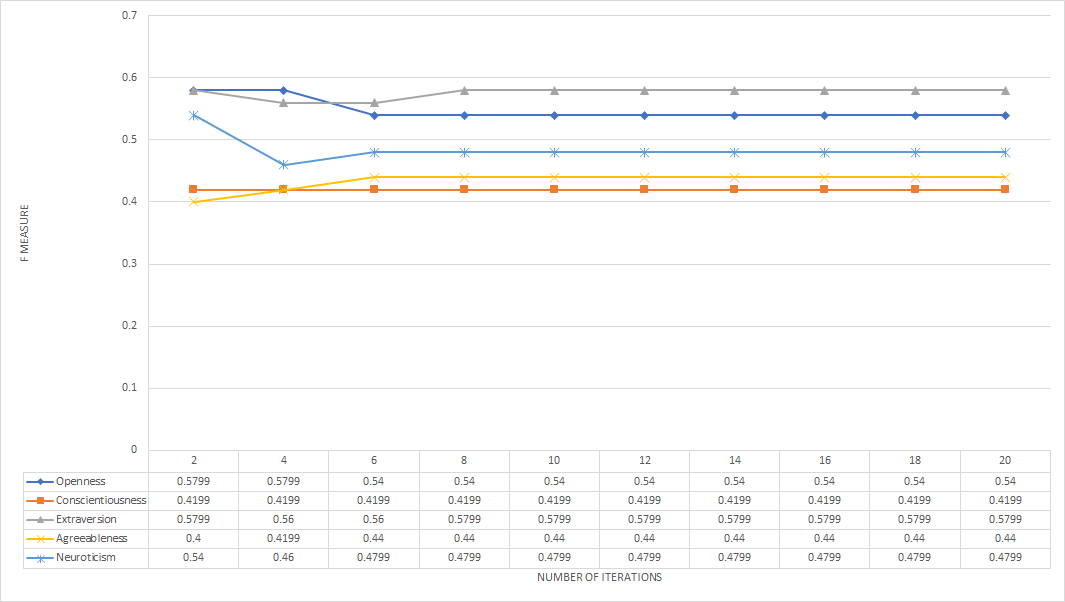
\includegraphics[width = \textwidth ]{fig/f-measure_logistic.png}
\caption{F-Measure vs Number of Iterations (Logistic Regression)}
\label{fig:f-measure_logistic}
\end{figure}


The followings tables show the confusion matrix of Naive Bayes for Big Five Personality classes:
\begin{table}[!ht]
\centering
\begin{tabular}{ |c|c|c| }
 \hline
 N =50 & Predicted:Yes & Predicted: No \\
 \hline
 Actual:Yes&4 & 11 \\
 \hline
 Actual:No&12 & 23 \\
 \hline
\end{tabular}
\caption{Confusion Matrix of Logistic Regression Model (Openness)}

\end{table}

\begin{table}[!ht]
\centering
\begin{tabular}{ |c|c|c| }
 \hline
 N =50 & Predicted:Yes & Predicted: No \\
 \hline
 Actual:Yes&6 & 18 \\
 \hline
 Actual:No&11 & 15 \\
 \hline
\end{tabular}
\caption{Confusion Matrix of Logistic Regression Model (Conscientiousness)}
\end{table}

\begin{table}[!ht]
\centering
\begin{tabular}{ |c|c|c| }
 \hline
 N =50 & Predicted:Yes & Predicted: No \\
 \hline
 Actual:Yes&22 & 9 \\
 \hline
 Actual:No&12 & 7 \\
 \hline
\end{tabular}
 \caption{Confusion matrix of Logistic Regression Model (Extraversion)}
\end{table}

\begin{table}[!ht]
\centering
\begin{tabular}{ |c|c|c| }
 \hline
 N =50 & Predicted:Yes & Predicted: No \\
 \hline
 Actual:Yes&9 & 14 \\
 \hline
 Actual:No&14 & 13 \\
 \hline
\end{tabular}
 \caption{Confusion Matrix of Logistic Regression Model (Agreeableness)}
\end{table}

\begin{table}[!h]
\centering
\begin{tabular}{ |c|c|c| }
 \hline
 N =50 & Predicted:Yes & Predicted: No \\
 \hline
 Actual:Yes&16 & 14 \\
 \hline
 Actual:No&12 & 8 \\
 \hline
\end{tabular}
 \caption{Confusion matrix of Logistic Regression Model (Neuroticism)}
\end{table}


\cleardoublepage
\subsection{Naive Bayes Model}
The following figure shows f-measure of the naive bayes model for Big Five Personality classes:
\begin{figure}[!ht]
\centering
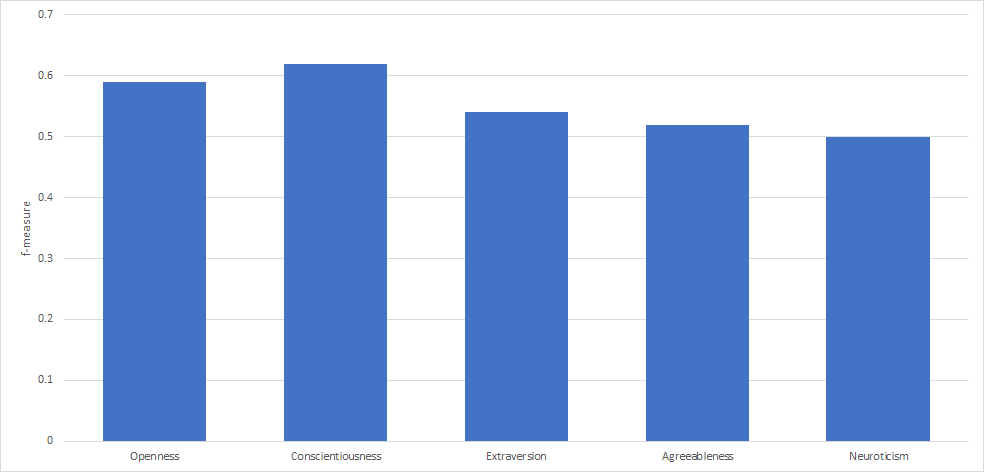
\includegraphics[width = \textwidth ]{fig/f-measure_naivebayes.png}
\caption{F-Measure of Naive Bayes Model}
\label{fig:f-measure_naivebayes}
\end{figure}

The followings tables show the confusion matrix of Naive Bayes for Big Five Personality classes:
\begin{table}[!ht]
\centering
\begin{tabular}{ |c|c|c| }
 \hline
 N =50 & Predicted:Yes & Predicted: No \\
 \hline
 Actual:Yes&3 & 12 \\
 \hline
 Actual:No&8 & 27 \\
 \hline
\end{tabular}
\caption{Confusion Matrix of Naive Bayes (Openness)}

\end{table}

\begin{table}[!ht]
\centering
\begin{tabular}{ |c|c|c| }
 \hline
 N =50 & Predicted:Yes & Predicted: No \\
 \hline
 Actual:Yes&9 & 15 \\
 \hline
 Actual:No&4 & 22 \\
 \hline
\end{tabular}
\caption{Confusion Matrix of Naive Bayes (Conscientiousness)}
\end{table}

\begin{table}[!ht]
\centering
\begin{tabular}{ |c|c|c| }
 \hline
 N =50 & Predicted:Yes & Predicted: No \\
 \hline
 Actual:Yes&20 & 11 \\
 \hline
 Actual:No&12 & 7 \\
 \hline
\end{tabular}
 \caption{Confusion Matrix of Naive Bayes (Extraversion)}
\end{table}

\begin{table}[!ht]
\centering
\begin{tabular}{ |c|c|c| }
 \hline
 N =50 & Predicted:Yes & Predicted: No \\
 \hline
 Actual:Yes&12 & 11 \\
 \hline
 Actual:No&13 & 14 \\
 \hline
\end{tabular}
 \caption{Confusion Matrix of Naive Bayes (Agreeableness)}
\end{table}

\begin{table}[!ht]
\centering
\begin{tabular}{ |c|c|c| }
 \hline
 N =50 & Predicted:Yes & Predicted: No \\
 \hline
 Actual:Yes&20 & 10 \\
 \hline
 Actual:No&15 & 5 \\
 \hline
\end{tabular}
 \caption{Confusion Matrix of Naive Bayes (Neuroticism)}
\end{table}


\subsection{Evaluation of Recommendation System}
The following table shows RMSE of various recommendation models:

  \begin{table}[!h]
	  \centering
    \begin{tabular}{| l | c |}
      \hline
      {\bf Recommendation Model} & {\bf RMSE}\\
      \hline
      User to User Collaborative Filtering with User & \\ Rating Matrix with combination of Global Baseline & 4.72\\
      \hline
      User to User Collaborative Filtering with User & \\ Rating Matrix & 3.89\\
      \hline
      User to User Collaborative Filtering with User & \\ Personality Matrix & 3.20\\
      \hline
      User to User Collaborative Filtering with Weighted & \\ Average of User Personality Matrix and User Rating Matrix & 3.2\\
      \hline
      User to User Collaborative Filtering with User & \\ Personality Matrix with combination of Global Baseline & 3.10\\
      \hline
      User to User Collaborative Filtering with Weighted & \\ Average of User Personality Matrix and User rating Matrix & \\ with combination of Global Baseline Algorithm & 3.04\\
      \hline
      Global Baseline Algorithm & 2.86\\
      \hline
      Matrix Factorization & 0.88\\
      \hline
    \end{tabular}
    \caption{RMSE of Recommendation System Models}
  \end{table}

The following figures show effects of change in number of nearest neighborhood in the different collaborative filtering models.\\

\begin{figure}[!ht]
  \centering
    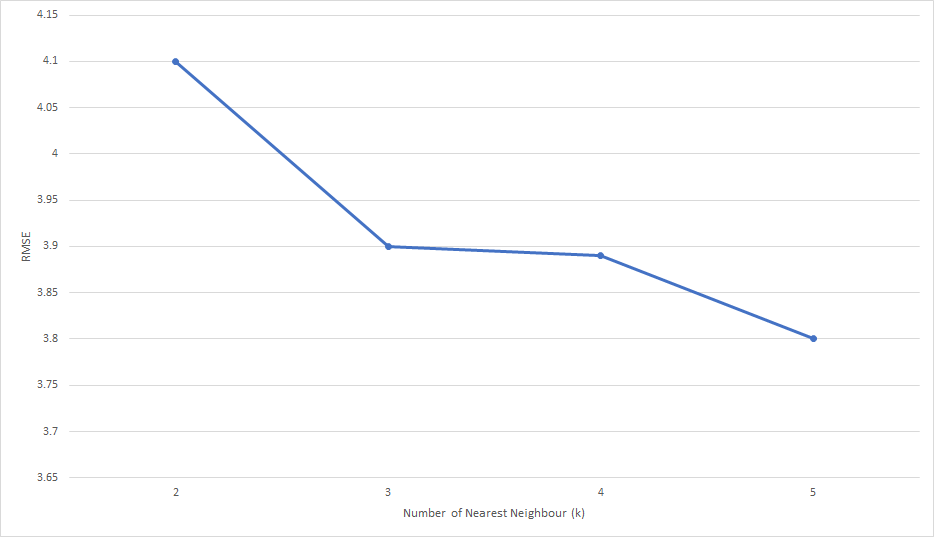
\includegraphics[width=1\textwidth]{fig/rmse_cf.png}
    \caption{RMSE of Collaborative Filtering with User Rating Matrix}
\end{figure}

\begin{figure}[!ht]
  \centering
    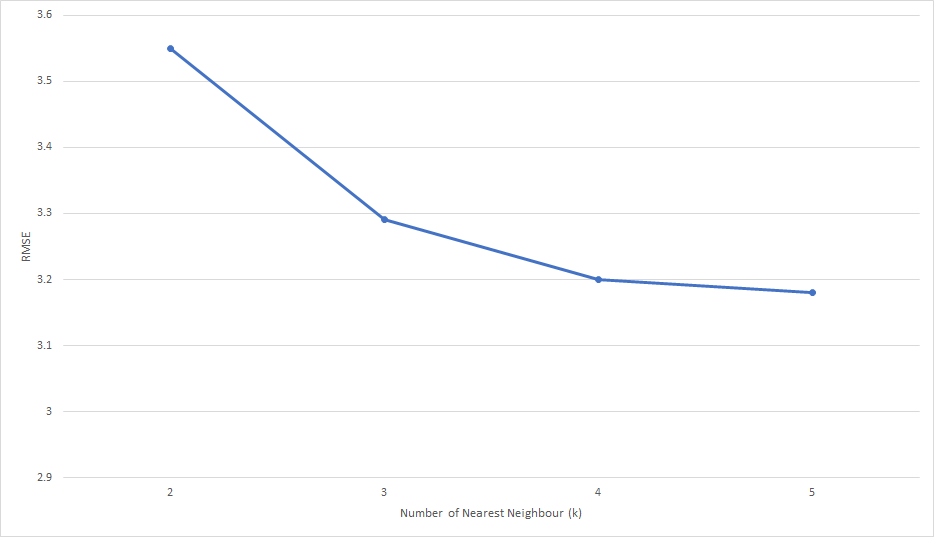
\includegraphics[width=1\textwidth]{fig/rmse_cf_personality.png}
    \caption{RMSE of Collaborative Filtering with similarity interm of Personality Matrix}
\end{figure}

\begin{figure}[!ht]
  \centering
    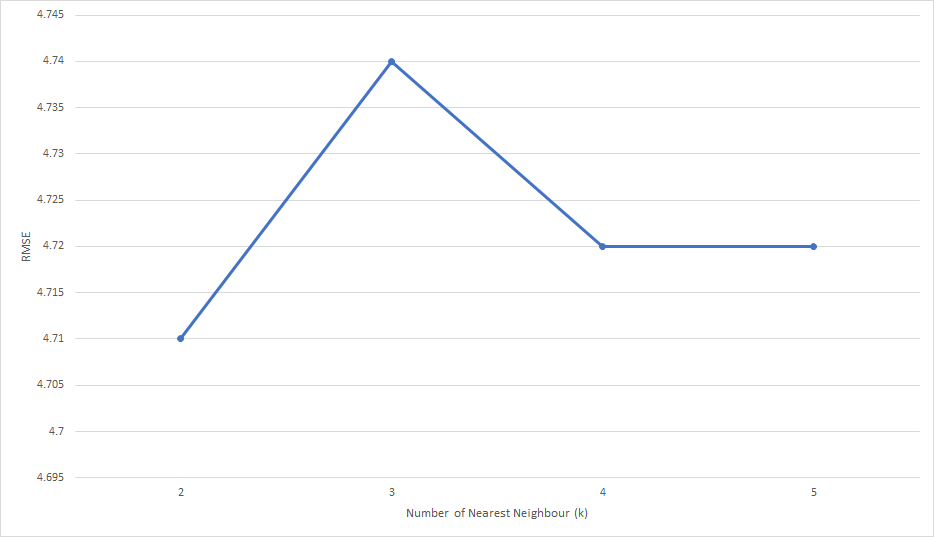
\includegraphics[width=1\textwidth]{fig/rmse_cf_global.png}
    \caption{RMSE of Collaborative Filtering combined with Global Baseline with User Rating Matrix}
\end{figure}

\begin{figure}[!ht]
  \centering
    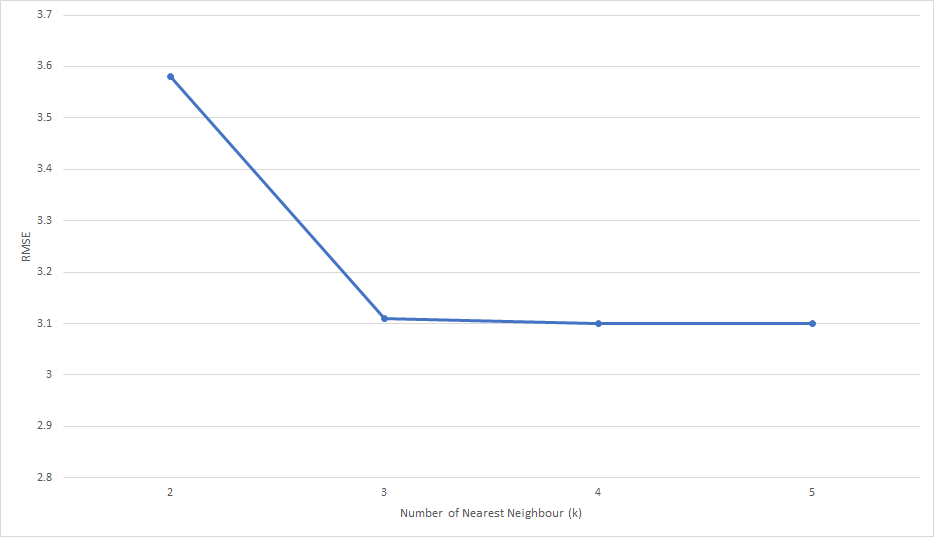
\includegraphics[width=1\textwidth]{fig/rmse_cf_global_personality.png}
    \caption{RMSE of Collaborative Filtering combined with Global Baseline with User Personality Matrix}
\end{figure}

\begin{figure}[!ht]
  \centering
    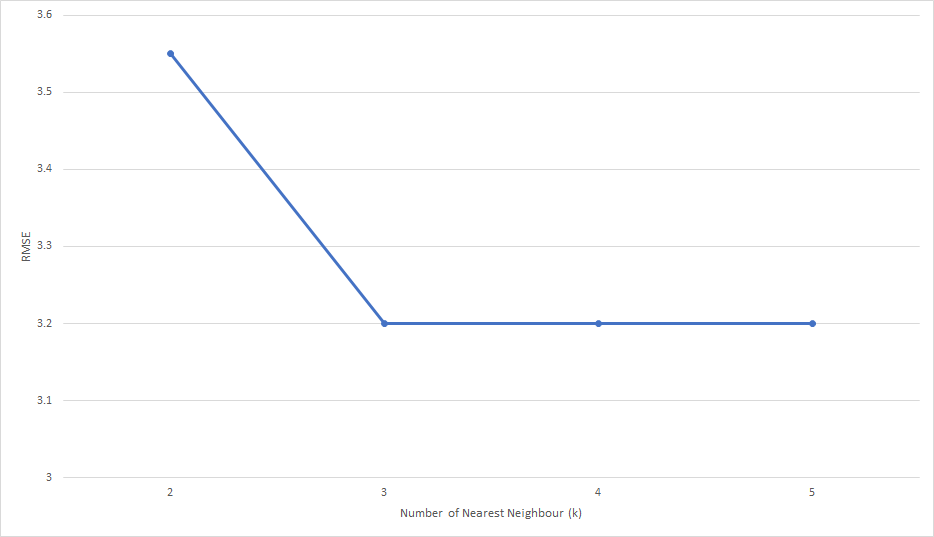
\includegraphics[width=1\textwidth]{fig/rmse_cf_average.png}
    \caption{RMSE of Collaborative Filtering with User Rating and Personality Matrix}
\end{figure}

\begin{figure}[!ht]
  \centering
    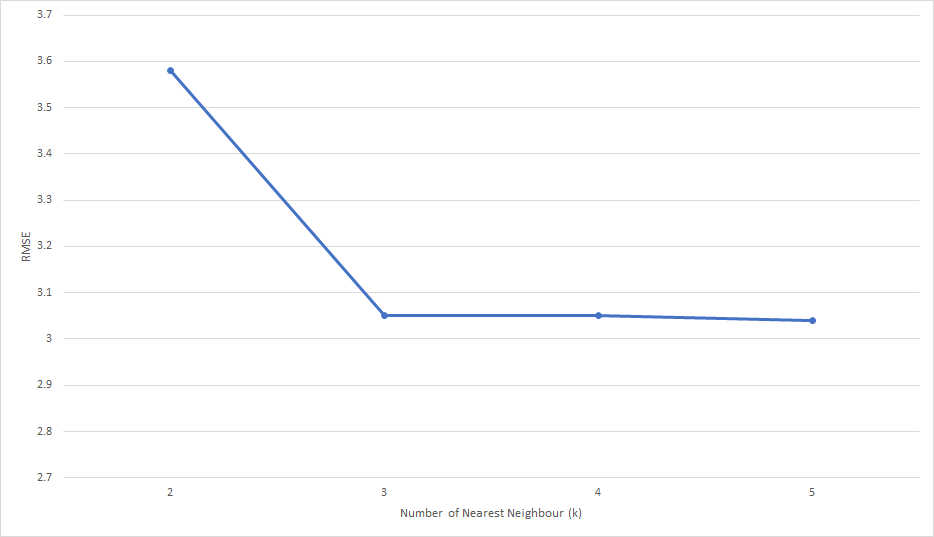
\includegraphics[width=1\textwidth]{fig/rmse_cf_combined_average.png}
    \caption{RMSE of Collaborative Filtering with User Rating and Personality Matrix combined with Global Baseline}
\end{figure}


\cleardoublepage
\subsubsection{Latent Factor}
The following figure shows the RMSE of matrix factorization when number of iterations is varied:

\begin{figure}[!ht]
\centering
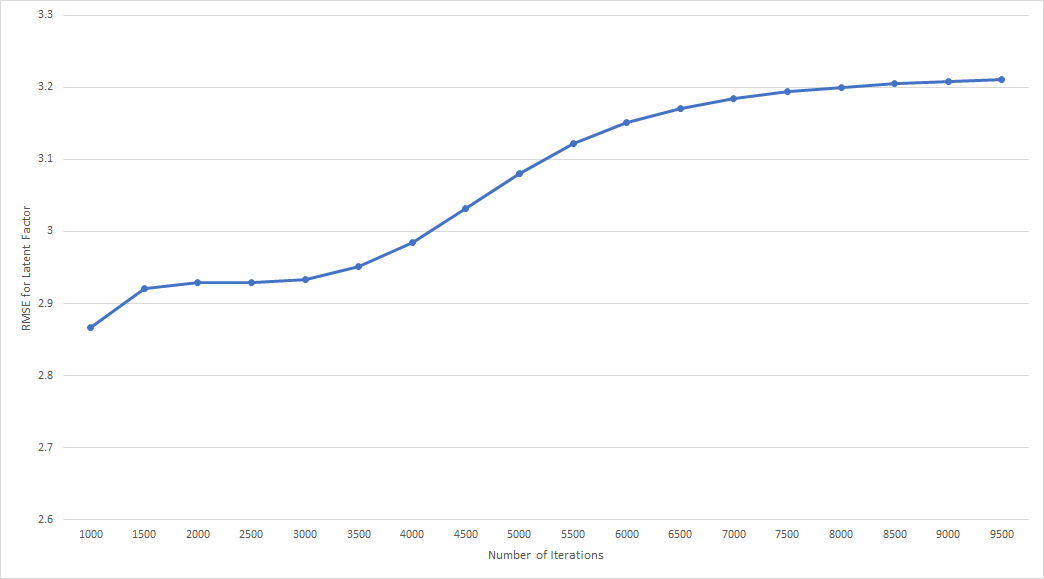
\includegraphics[width = 0.97\textwidth ]{fig/rmse_step.png}
\caption{RMSE of Matrix Factorization vs Number of Iterations}
\label{fig:rmse_step}
\end{figure}

The following figure shows the RMSE of matrix factorization when k is varied with number of iterations is fixed at 1000:
\begin{figure}[!ht]
\centering
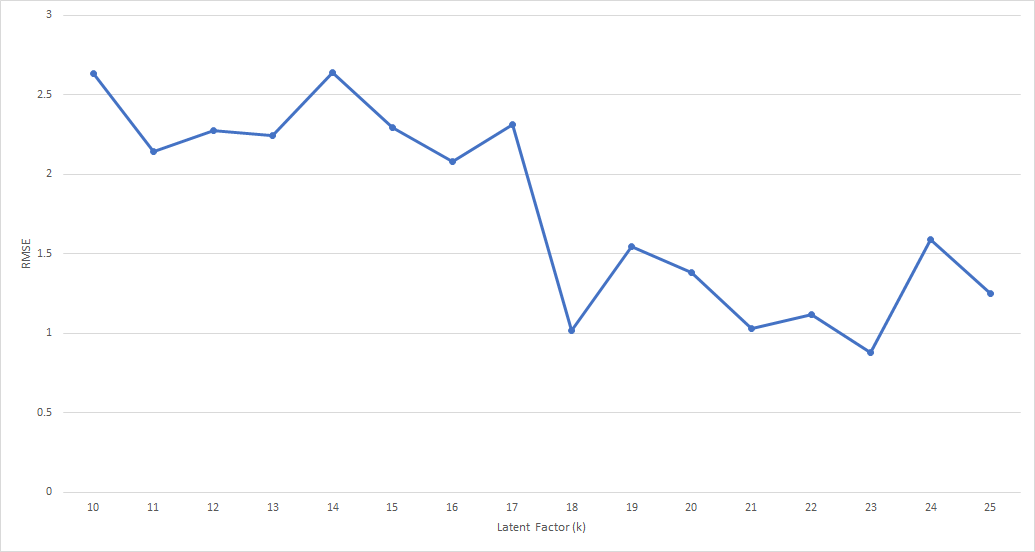
\includegraphics[width = 0.97\textwidth ]{fig/rmse_k.png}
\caption{RMSE of Matrix Factorization vs Number of Latent Factors}
\label{fig:rmse_k}
\end{figure}

Comparison of the above models, we can conclude that the result of user to user collaborative filtering with the personality has slightly better result than the user to user collaborative filtering with the user Rating matrix but the matrix factorization outperforms them all. Besides, the result of weighted average of user similarity matrix with rating and personality also performs better than only a rating matrix but has a comparable result with the user to user collaborative filtering with personality to compute the similarity. Currently the system uses \textbf{switching hybrid} methodology in order to recommend the user among the different models used in the system i.e one with the least RMSE.
